\documentclass[../main.tex]{subfiles}

\begin{document}
\chapter{The Charged Particle Data Processing Library LANDO}
LANDO is a C++ charged particle data processing code that produces JSON formatted multigroup charged particle data from ENDF files. Figure \ref{fig:LANDO_code_structure} shows the general code structure and data processing method that LANDO uses; in general LANDO first reconstructs the charged particle cross sections using the \textbf{Construct} class and a \textit{screening} function. Next LANDO interprets the constructed cross sections into light/heavy reactions using the \textbf{Interpret} class using the Boltzmann-Fokker-Planck (BFP) \textit{decomposition} functions. Finally, LANDO generates the multigroup data from the interpretation by using the \textbf{Multigroup} class and a \textit{weighting} function.

\begin{figure}[!htb]
\centering
\resizebox{0.5\columnwidth}{!}{%
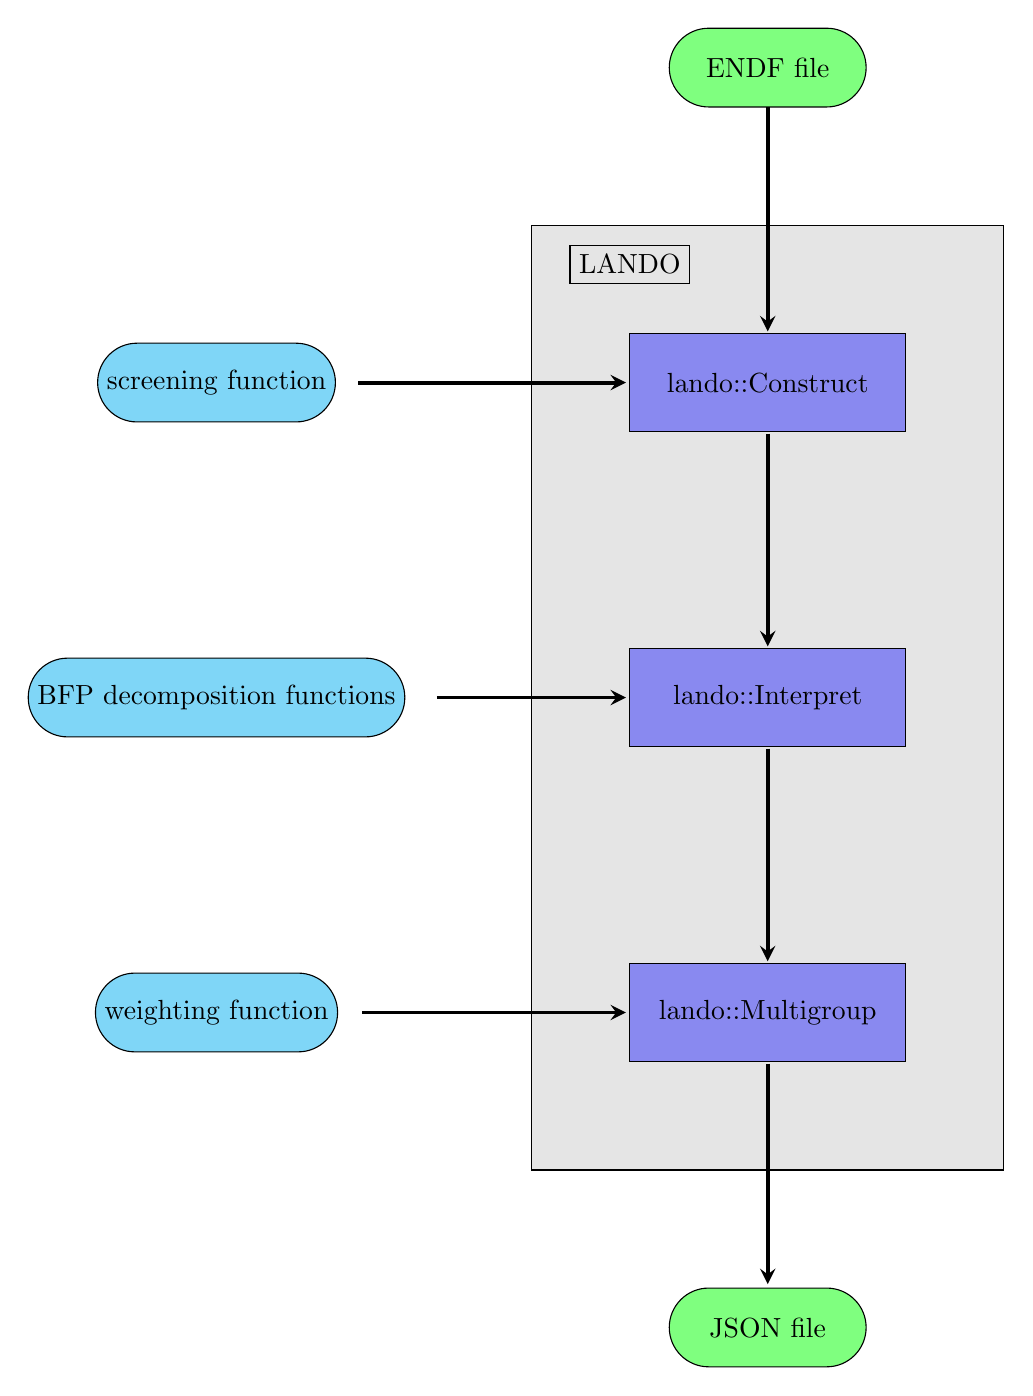
\begin{tikzpicture}
  % LANDO Code
  \node[draw,
    minimum width=6cm,
    minimum height=12cm,
    fill=lightgray,
    fill opacity=0.4] (PProcess) at (0,-4) {};
    
  % ENDF file
  \node[draw,
    rounded corners=0.5cm,
    minimum width=2.5cm,
    minimum height=1cm,
    fill=green,
    fill opacity=0.5,
    text opacity = 1] at (0,4){ENDF file};
    
  % Screening function
  \node[draw,
    rounded corners=0.5cm,
    minimum width=2.5cm,
    minimum height=1cm,
    fill=cyan,
    fill opacity=0.5,
    text opacity = 1] at (-7,0){screening function};
    
  % Construct.hpp
  \node[draw,
    minimum width=3.5cm,
    minimum height=1.25cm,
    outer sep=0,
    fill=blue,
    fill opacity=0.4,
    text opacity=1] (PProcess) at (0,0)  {lando::Construct};
  
  % BFP decomposition functions
  \node[draw,
    rounded corners=0.5cm,
    minimum width=2.5cm,
    minimum height=1cm,
    fill=cyan,
    fill opacity=0.5,
    text opacity = 1] at (-7,-4){BFP decomposition functions};
    
  % Interpret.hpp
  \node[draw,
    minimum width=3.5cm,
    minimum height=1.25cm,
    outer sep=0,
    fill=blue,
    fill opacity=0.4,
    text opacity=1] (PProcess) at (0,-4)  {lando::Interpret};
  
  % Weighting functions
  \node[draw,
    rounded corners=0.5cm,
    minimum width=2.5cm,
    minimum height=1cm,
    fill=cyan,
    fill opacity=0.5,
    text opacity = 1] at (-7,-8){weighting function};
    
  % Multigroup.hpp
  \node[draw,
    minimum width=3.5cm,
    minimum height=1.25cm,
    outer sep=0,
    fill=blue,
    fill opacity=0.4,
    text opacity=1] (PProcess) at (0,-8)  {lando::Multigroup};
  
  % JSON file
  \node[draw,
    rounded corners=0.5cm,
    minimum width=2.5cm,
    minimum height=1cm,
    fill=green,
    fill opacity=0.5,
    text opacity = 1] at (0,-12){JSON file};
  
  % Draw Arrows
  \draw[-stealth, line width=0.50mm] (0.0, 3.5) -- (0.0, 0.65);
  \draw[-stealth, line width=0.50mm] (-5.2, 0.0) -- (-1.8, 0.0);
  \draw[-stealth, line width=0.50mm] (0.0,-0.65) -- (0.0,-3.35);
  \draw[-stealth, line width=0.50mm] (-4.2,-4) -- (-1.8,-4);
  \draw[-stealth, line width=0.50mm] (0.0,-4.65) -- (0.0,-7.35);
  \draw[-stealth, line width=0.50mm] (-5.15, -8) -- (-1.8, -8);
  \draw[-stealth, line width=0.50mm] (0.0,-8.65) -- (0.0,-11.45);
  
  % Text labels
  \node[draw] at (-1.75,1.5) {LANDO};
 
\end{tikzpicture}
}
\caption{Flow chart describing the general structure of LANDO}
\label{fig:LANDO_code_structure}
\end{figure}

The remainder of this documentation describes the classes \textbf{Construct}, \textbf{Interpret}, and \textbf{Multigroup}, and the auxiliary functions needed by these classes. First the classes are described in detail, and then the auxiliary functions are discussed.

\section{Construct class}
The construct class in LANDO reconstructs all of the cross sections available in an ENDF file according to the ENDF manual. This is done for both the total cross sections (MF3) and the differential cross sections (MF6). The class is templated on a labmda function that serves as the screening function for the Coulomb differential cross section. For example, to construct the cross sections for deuterium-tritium system from the availible ENDF file, the Construct class would be constructed as:

\begin{lstlisting}
 #include "Lando.hpp"

 auto screening = lando::screening::none();
 lando::Construct<decltype(screening)> data("d-001_H_002.endf", screening);
\end{lstlisting}

Once an ENDF file has been reconstructed, the following methods are available to the following return sub-classes:

\begin{lstlisting}
 using construct = lando::Construct<decltype(screening)>;
  
 Construct::MF1 mf1 = data.generalInformation();
 std::vector<construct::MF3> mf3 = data.reactionCrossSections();
 std::vector<construct::MF6> mf6 = data.productEnergyAngleDistributions();
\end{lstlisting}

The following subsections describe each of the sub-classes, and the methods within each sub-class to access the information and reconstructed cross sections.

\subsection{General information}
The general information class provides the same general information about the reaction as the original ENDF file. The following methods are available:
\begin{lstlisting}
 auto  ZA = mf1.ZA();
 auto ZAI = mf1.ZAI();
  
 auto AWR = mf1.AWR();
 auto AWR = mf1.materialAtomicMassRatio();

 auto LRP = mf1.LRP();
 auto LRP = mf1.resonanceParameterFlag();

 auto LFI = mf1.LFI();
 auto LFI = mf1.isFissile();

 auto NLIB = mf1.NLIB();
 auto NLIB = mf1.libraryType();

 auto NMOD = mf1.NMOD();
 auto NMOD = mf1.modificationNumber();

 auto ELIS = mf1.ELIS();
 auto ELIS = mf1.excitationEnergy();

 auto STA = mf1.STA();
 auto STA = mf1.isStable();

 auto LIS = mf1.LIS();
 auto LIS = mf1.excitedLevel();

 auto LISO = mf1.LISO();
 auto LISO = mf1.isomericLevel();

 auto NFOR = mf1.NFOR();
 auto NFOR = mf1.libraryFormat();

 auto AWI = mf1.AWI();
 auto AWI = mf1.projectileAtomicMassRatio();

 auto EMAX = mf1.EMAX();
 auto EMAX = mf1.maximumEnergy();

 auto LREL = mf1.LREL();
 auto LREL = mf1.releaseNumber();

 auto NSUB = mf1.NSUB();
 auto NSUB = mf1.subLibrary();

 auto NVER = mf1.NVER();
 auto NVER = mf1.versionNumber();

 auto TEMP = mf1.TEMP();
 auto TEMP = mf1.temperature();

 auto RTOL = mf1.RTOL();
 auto RTOL = mf1.reconstructionTolerance();

 auto LDRV = mf1.LDRV();
 auto LDRV = mf1.derivedMaterial();
\end{lstlisting}


\subsection{Reaction cross sections}
The reaction cross section provides the angle-integrated reaction cross sections for each reaction in an ENDF file. The following general information is provided for each reaction:
\begin{lstlisting}
 auto reaction = mf3[0];

 auto energies = reaction.energies();
 auto values = reaction.values();
 auto interpolations = reaction.interpolations();
 auto interpolationBounds = reaction.interpolationBounds();
 auto QI = reaction.QI();
 auto QM = reaction.QM();

 auto MT = reaction.MT();
 auto ZA = reaction.ZA();
 auto AWR = reaction.AWR();
 auto ZAI = reaction.ZAI();
 auto AWI = reaction.AWI();
\end{lstlisting}

This class also provides a method to access the angle-integrated reaction cross section that takes an energy in MeV and returns the cross section in barns, see the following example:
\begin{lstlisting}
  double E = 1.0; // MeV
  auto sigma = reaction.sigma(E); // barns
\end{lstlisting}

\subsection{Energy-angle distributions}
The \textbf{Energy-angle distributions} sub-class reconstructs the differential cross sections for File 6 in the ENDF files. This sub-class requires information from both the \textbf{Information} and \textbf{Reaction cross sections} sub-classes to be able to reconstruct the differential cross sections. The differential cross section for any reaction are defined in the ENDF files by giving the production cross section for each reaction product in barns/steradian assuming azimuthal symmetry:
\begin{equation} \label{eqn:differential-cross-section}
    \sigma_i(E^{\prime},E,\mu_0) = \sigma(E^{\prime}) \, y_i(E^{\prime}) \, f_i(E^{\prime},E,\mu_0) / 2\, \pi
\end{equation}
where:
\begin{align*}
    i \quad & \text{denotes one particular product} \\
    E^{\prime} \quad & \text{is the incident energy} \\
    E \quad & \text{is the energy of the product emitted with cosine of scattering $\mu_0$} \\
    \sigma(E^{\prime}) \quad & \text{is the reaction cross section} \\
    y_i(E^{\prime}) \quad & \text{is the product yield or multiplicity for particle $i$} \\
    f_i \quad & \text{is the normalized distribution with units $(\text{eV}\cdot \text{unit-cosine})^{-1}$ }
\end{align*}

For each possible reaction (MT) that exists in the ENDF file, LANDO reconstructs the differential cross section for all products. The product differential cross section are represented in the ENDF using seven different representations (law's in ENDF), they are:
\begin{itemize}
    \item LAW 0: Unknown distribution
    \item LAW 1: Continuum energy-angle distribution
    \item LAW 2: Discrete two-body scattering
    \item LAW 3: Isotropic discrete emission
    \item LAW 4: Discrete two-body recoils
    \item LAW 5: Charged particle elastic scattering
    \item LAW 6: N-body phase space
    \item LAW 7: Laboratory angle-energy
\end{itemize}
Hence, each reactions possible differential cross sections are tabulated as a vector of a variant of all seven distribution types. The following code snippet demonstrates how to access a specific reactions differential cross sections:

\begin{lstlisting}
 #include "Lando.hpp"

 /* Construct the cross sections */
 auto screening = lando::screening::none();
 lando::Construct<decltype(screening)> data("d-001_H_002.endf", screening);
 
 /* Define te various LAWS */
 using LAW0 = decltype(data)::MF6::Unknown;
 using LAW1 = decltype(data)::MF6::ContinuumEnergyAngle;
 using LAW2 = decltype(data)::MF6::DiscreteTwoBodyScattering;
 using LAW3 = decltype(data)::MF6::IsotropicDiscreteEmission;
 using LAW4 = decltype(data)::MF6::DiscreteTwoBodyRecoils;
 using LAW5 = decltype(data)::MF6::ChargedParticleElasticScattering;
 using LAW6 = decltype(data)::MF6::NBodyPhaseSpace;
 using LAW7 = decltype(data)::MF6::LaboratoryAngleEnergy;
 
 /* Define the type of the products in MF6 */
 using Product = std::variant< LAW0, LAW1, LAW2, LAW3, LAW4, LAW5, LAW6, LAW7 >;
 
 /* Get the energy-angle distributions */                  
 std::vector< decltype(data)::MF6 > differentialCrossSections 
    = data.productEnergyAngleDistributions();
    
 /* Get a specific reaction */
 std::vector< Product > crossSection = differentialCrossSections[0];
\end{lstlisting}

To access a specific cross section within the vector of distributions, one should use \textbf{std::visit} in combination with \textbf{njoy::utility::overload} where lambda functions for each of the types in the previous code snippet are defined. The following code snippet demonstrates this
\begin{lstlisting}
 /* Starting with crossSection from previous code snippet */ 
 std::visit( njoy::utility::overload{ 
        [] (const LAW0& ) {},
        [] (const LAW1& ) {},
        [] (const LAW2& ) {},
        [] (const LAW3& ) {}, 
        [] (const LAW4& ) {},
        [] (const LAW5& ) {}, 
        [] (const LAW6& ) {},
        [] (const LAW7& ) {} },
    crossSection[0] );
\end{lstlisting}

Every cross section has the following base methods available to help identify the specific the reaction occuring:
\begin{lstlisting}
 /* Starting with a specific cross section from previous code snippet */
 LAW crossSection = std::get< LAW >(differentialCrossSections[0]); // LAW is 0-7
 
 auto  MT = crossSection.MT(); // ENDF reaction identifier

 auto ZAI = crossSection.ZAI(); // ZIAD of incident particle
 auto  ZA = crossSection.ZA();  // ZIAD of target particle 
 auto ZAP = crossSection.ZAP(); // ZIAD of emitted particle

 auto AWI = crossSection.AWI(); // Weight of incident particle
 auto AWR = crossSection.AWR(); // Weight of target particle
 auto AWP = crossSection.AWP(); // Weight of emitted particle
  
 auto LIP = crossSection.LIP(); // ENDF product modifier
 auto LAW = crossSection.LAW(); // Distribution type of cross section
\end{lstlisting}

Additionally, for every distribution the method \textbf{sigma} is provided which returns the value of the differential cross at the energies angle specified. For two-body interactions, \textbf{sigma} is only a function of the incident energy in the LAB frame and cosine of the CM scattering angle; for multi-body reactions, \textbf{sigma} is a function of the incident energy in the LAB frame, cosine of the CM scattering angle for the product, and the outgoing energy of the product in the LAB frame.
\begin{lstlisting}
 /* Starting with a cross section from previous code snippet */
 auto value1 = crossSection.sigma(5.0, 0.25); // Two-body reaction
 
 auto value2 = crossSection.sigma(5.0, 4.0, 0.25); // Multi-body reaction
\end{lstlisting}
In the remainder of this section the methods by which each of the seven possible distribution types are used to reconstruct the normailizied distributions in Eq. \eqref{eqn:differential-cross-section} are discussed. 

% \subsection{LAW 0: Unknown}
% Not implemented.

% \subsection{LAW 1: Continuum energy angle}
% This distribution is used to describe particles emitted in multi-body reactions or combinations of several reactions, such as scattering through a range of levels or reactions at high energies where many channels are normally open.

% \subsubsection{Legendre coefficients representations}
% Legendre coefficients are used as follows:
% \begin{equation}
%     f(E^{\prime},E,\mu_0) = \sum_{l=0}^{NA} \dfrac{2l + 1}{2} \, f_l(E^{\prime},E) \, P_l(\mu_0)
% \end{equation}
% where NA is the number of angular parameters. 

% \subsubsection{Kalbach-Mann systematics representation}
% Kalbach-Mann systematics are a powerful representation for outgoing neutron and charged particle energy-angle distributions in high energy (usually pre-equilibrium) reactions. The Kalbach-Mann formulation addresses reactions of the form 
% \begin{equation}
%     a + A = C = B + b
% \end{equation}
% where:
% \begin{align*}
%     a \quad &\text{is the incident projectile}, \\
%     A \quad &\text{is the target nucleus}, \\
%     C \quad &\text{is the compound nucleus}, \\
%     b \quad &\text{is the emitted particle}, \\
%     B \quad &\text{s the residual nucleus}.
% \end{align*}

% The double differential distribution for projectiles other than photons is
% \begin{equation}
%     f(E_a,E_b^C,\mu_0) = \dfrac{a \, f_0}{2 \, \sinh{a}} \Big[ \cosh \left(a \, \mu_0\right) + r \, \sinh \left(a \, \mu_0\right) \Big]
% \end{equation}
% where:
% \begin{align*}
%     E_a   \quad &\text{is the energy of the incident projectile a in the laboratory system}, \\
%     E_b^C \quad &\text{is the energy of the emitted particle in the CM system}, \\
%     \mu_0 \quad &\text{is the cosine of the scattering angle of the emitted particle b in the CM system}, \\
%     a     \quad &\text{is a simple parameterized function }, \\
%     f_0   \quad &\text{is the total emission probability}, \\
%     r     \quad &\text{is the pre-compound fraction as given by the evaluator.} \\
% \end{align*}

% The formula for calculating the slope value $a = a(E_a, E_b^C)$ is:
% \begin{equation}
%     a = C_1 \, X_1 + C_2 \, X_1^3 + C_3 \, M_a \, m_b \, X_3^4
% \end{equation}
% where:
% \begin{equation*}
%     \begin{split}
%         e_a &= \epsilon_a + S_a \\
%         R_1 &= \min(e_a, E_{t1}) \\
%         X_1 &= R_1 \, e_b / e_a
%     \end{split}
%     \quad\quad\quad\quad\quad
%     \begin{split}
%         e_b &= \epsilon_b + S_b \\
%         R_3 &= \min(e_a, E_{t3}) \\
%         X_3 &= R_3 \, e_b / e_a
%     \end{split}
% \end{equation*}
% The parameter values for light particle induced reactions are:
% \begin{equation*}
%     \begin{split}
%         \epsilon_a &= E_a \left(\dfrac{\text{AWR}_A}{\text{AWR}_A + \text{AWR}_a}\right) \\
%         C_1 &= 0.04 / \text{MeV} \\
%         C_3 &= 6.7 \cdot 10^{-7} / (\text{MeV})^4 \\
%         E_{t1} &= 130 \text{MeV} \\
%         M_n &= 1 \\
%         M_d &= 1 \\
%         m_n &= 1/2 \\
%         m_d &= 1 \\
%         m_{He-3} &= 1
%     \end{split}
%     \quad\quad\quad\quad\quad
%     \begin{split}
%         \epsilon_b &= E_b^C \left(\dfrac{\text{AWR}_B + \text{AWR}_b}{\text{AWR}_B} \right)\\
%         C_1 &= 1.8 \cdot 10^{-6} / (\text{MeV})^3 \\
%         \\
%         E_{t3} &= 41 \text{MeV} \\
%         M_p &= 1 \\
%         M_{\alpha} &= 0 \\
%         m_p &= 1 \\
%         m_t &= 1 \\
%         m_{\alpha} &= 2
%     \end{split}
% \end{equation*}
% Note that Kalbach never specified $M_t$ or $M_{He-3}$ as the systematics have not been extended to high energy t and 3He projectiles, where the $X_3$ term contributes.

% $S_a$ and $S_b$ are the separation energies for the incident and emitted particles, respectively, for the reaction $A + a \rightarrow C \rightarrow B + b$. As the particle emission is occuring for relatively high energies, pairing and shell effects in the compound nucleus are muted and must be neglected in the calculation of separation energies. Therefore, one should use the following formulae for the separation energies3 in MeV:
% \begin{multline}
%     S_a = 15.68 \left[ A_C - A_A \right] - 28.07 \left[ \dfrac{(N_C - Z_C)^2}{A_C} - \dfrac{(N_A - Z_A)^2}{A_A} \right] \\
%     - 18.56 \left[ A_C^{2/3} - A_A^{2/3} \right] + 33.22 \left[ \dfrac{(N_C - Z_C)^2}{A_C^{4/3}} - \dfrac{(N_A - Z_A)^2}{A_A^{4/3}} \right] \\
%     - 0.717 \left[ \dfrac{Z_C^2}{A_C^{1/3}} - \dfrac{Z_A^2}{A_A^{1/3}} \right] + 1.211 \left[ \dfrac{Z_C^2}{A_C} - \dfrac{Z_A^2}{A_A} \right] - I_a
% \end{multline}
% and
% \begin{multline}
%     S_a = 15.68 \left[ A_C - A_B \right] - 28.07 \left[ \dfrac{(N_C - Z_C)^2}{A_C} - \dfrac{(N_B - Z_B)^2}{A_B} \right] \\
%     - 18.56 \left[ A_C^{2/3} - A_B^{2/3} \right] + 33.22 \left[ \dfrac{(N_C - Z_C)^2}{A_C^{4/3}} - \dfrac{(N_B - Z_B)^2}{A_B^{4/3}} \right] \\
%     - 0.717 \left[ \dfrac{Z_C^2}{A_C^{1/3}} - \dfrac{Z_B^2}{A_B^{1/3}} \right] + 1.211 \left[ \dfrac{Z_C^2}{A_C} - \dfrac{Z_B^2}{A_B} \right] - I_b
% \end{multline}
% where:
% \begin{align*}
%     A,B,C   \quad &\text{subscripts for the target, residual, and compound nuclei respectively}, \\
%     N, Z, A  \quad &\text{are the neutron, proton, and mass numbers of each nuclei}, \\
%     I_a, I_b \quad &\text{are the energies required to separate the incident and emitted particles}.
% \end{align*}

% \subsection{LAW 2: Discrete two-body scattering}
% This law is used to describe the distribution in energy and angle of particles described by two-body kinematics. Since the energy of a particle emitted with a particular scattering cosine $\mu_0$ is determined by kinematics (see chapter 1), it is only necessary to give:
% \begin{equation} \label{eqn:law2-legendre}
%     p_i(E^{\prime}, \mu_0) = \int dE \, f_i(E^{\prime},E,\mu_0) = \dfrac{1}{2}+ \sum\limits_{\ell = 1}^L \dfrac{2\ell + 1}{2} \, a_{\ell}(E{\prime}) \, P_{\ell}(\mu_0)
% \end{equation}
% where the $P_{\ell}$ are the Legendre polynomials with the maximum order $L$, and $a_{\ell}(E)$ are the Legendre coefficients at energy $E$. In ENDF files the data is given as seta of $E_i^{\prime}$ and $a_{i,\ell}$ values. To reconstruct the differential cross section: one first find the appropriate energy bin and reconstructs the values $(E_i^{\prime}, p_i)$ and $(E_{i+1}^{\prime}, p_{i+1})$ using the Eq. \eqref{eqn:law2-legendre}. Then one interpolates for the value $(E^{\prime}, p)$ using the appropriate interpolation technique as defined by the reaction (see Chapter 2 for interpolation methods).

% \subsection{LAW 3: Isotropic discrete emission}
% The cross section is the same as LAW 2 except there is no angular distribution. Therefore the differential cross section is simply:
% \begin{equation}
%     \sigma_i(E^{\prime}) = \sigma(E^{\prime}) \, y_i(E^{\prime})
% \end{equation}

% \subsection{LAW 4: Discrete two-body recoils}
% If the recoil nucleus of a two-body reaction does not break up, its energy and angular distribution can be determined from the kinematics. For these type of reactions ENDF files contain no LAW dependent structure, and it is upto the user to reconstruct these differential cross sections. This is straight forward to do because the cosine of the CM recoil angle, $\eta_0$, is simply equal to minus the cosine of the CM scattering angle $\mu_0$; therefore these cross section are simply
% \begin{equation}
%     f_{LAW 4}(E^{\prime},\eta_0) = f_{LAW 2}(E^{\prime}, -\mu_0).
% \end{equation}

% \subsection{LAW 5: Charged particle elastic scattering}
% Elastic scattering of charged particles includes components from Coulomb scattering, nuclear scattering, and the interference between them. The screened Coulomb differential cross sections for distiguishible and identical particles are derived in Chapter 3. The total differential cross section is written as
% \begin{equation}
%     \sigma_{el}(E^{\prime},\mu_0) = \sigma_{C}(E^{\prime},\mu_0) + \sigma_{N}(E^{\prime},\mu_0) + \sigma_{I}(E^{\prime},\mu_0),
% \end{equation}
% where the subscripts $C$, $N$, and $I$ represent the Coulomb, nuclear-elastic scattering, and interference parts of the differential cross section.

% \subsection{LAW 6: N-body phase space}
% In the absence of detailed information, it is often useful to use n-body phase-space distributions for the particles emitted from neutron and charged-particle reactions. These distributions conserve energy and momentum, and they provide reasonable kinematic limits for secondary energy and angle in the LAB system. Note, LAW 6 is meant for situations where the number of emitted particles is $\geq 3$. In the CM system, the phase-space distribution for particle i is
% \begin{equation}
%     p_i^{CM}(E^{\prime},E,\mu_0) = C_n \, \sqrt{E} \, \left(E_i^{\text{max}} - E\right)^{(3n/2)-4}
% \end{equation}
% where $E_i^{\text{max}}$ is the maximum possible CM energy for particle $i$, and $C_n$ are the normalization coefficients
% \begin{align*}
%     C_3 &= \dfrac{4}{\pi \, (E_i^{\text{max}})^2}\\
%     C_4 &= \dfrac{105}{32 \, (E_i^{\text{max}})^{7/2}} \\
%     C_5 &= \dfrac{256}{14 \, \pi \, (E_i^{\text{max}})^5}
% \end{align*}

% The value of $E_i^{\text{max}}$ is a fraction of the energy availible i CM,
% \begin{equation}
%     E_i^{\text{max}} = \dfrac{M - m_i}{M} E_a
% \end{equation}
% where $M$ is the total mass of the $n$ particles being treated by the law.

% \subsection{LAW 7: Laboratory angle-energy}
% Not implemented.

\section{Interpret Class}

\section{Multigroup Class}

\section{Examples}
\end{document}